\documentclass[]{book}
\usepackage{lmodern}
\usepackage{amssymb,amsmath}
\usepackage{ifxetex,ifluatex}
\usepackage{fixltx2e} % provides \textsubscript
\ifnum 0\ifxetex 1\fi\ifluatex 1\fi=0 % if pdftex
  \usepackage[T1]{fontenc}
  \usepackage[utf8]{inputenc}
\else % if luatex or xelatex
  \ifxetex
    \usepackage{mathspec}
  \else
    \usepackage{fontspec}
  \fi
  \defaultfontfeatures{Ligatures=TeX,Scale=MatchLowercase}
\fi
% use upquote if available, for straight quotes in verbatim environments
\IfFileExists{upquote.sty}{\usepackage{upquote}}{}
% use microtype if available
\IfFileExists{microtype.sty}{%
\usepackage{microtype}
\UseMicrotypeSet[protrusion]{basicmath} % disable protrusion for tt fonts
}{}
\usepackage[margin=1in]{geometry}
\usepackage{hyperref}
\hypersetup{unicode=true,
            pdftitle={Introduction to Bioinformatics},
            pdfauthor={Diego Diez},
            pdfborder={0 0 0},
            breaklinks=true}
\urlstyle{same}  % don't use monospace font for urls
\usepackage{natbib}
\bibliographystyle{apalike}
\usepackage{color}
\usepackage{fancyvrb}
\newcommand{\VerbBar}{|}
\newcommand{\VERB}{\Verb[commandchars=\\\{\}]}
\DefineVerbatimEnvironment{Highlighting}{Verbatim}{commandchars=\\\{\}}
% Add ',fontsize=\small' for more characters per line
\usepackage{framed}
\definecolor{shadecolor}{RGB}{248,248,248}
\newenvironment{Shaded}{\begin{snugshade}}{\end{snugshade}}
\newcommand{\KeywordTok}[1]{\textcolor[rgb]{0.13,0.29,0.53}{\textbf{#1}}}
\newcommand{\DataTypeTok}[1]{\textcolor[rgb]{0.13,0.29,0.53}{#1}}
\newcommand{\DecValTok}[1]{\textcolor[rgb]{0.00,0.00,0.81}{#1}}
\newcommand{\BaseNTok}[1]{\textcolor[rgb]{0.00,0.00,0.81}{#1}}
\newcommand{\FloatTok}[1]{\textcolor[rgb]{0.00,0.00,0.81}{#1}}
\newcommand{\ConstantTok}[1]{\textcolor[rgb]{0.00,0.00,0.00}{#1}}
\newcommand{\CharTok}[1]{\textcolor[rgb]{0.31,0.60,0.02}{#1}}
\newcommand{\SpecialCharTok}[1]{\textcolor[rgb]{0.00,0.00,0.00}{#1}}
\newcommand{\StringTok}[1]{\textcolor[rgb]{0.31,0.60,0.02}{#1}}
\newcommand{\VerbatimStringTok}[1]{\textcolor[rgb]{0.31,0.60,0.02}{#1}}
\newcommand{\SpecialStringTok}[1]{\textcolor[rgb]{0.31,0.60,0.02}{#1}}
\newcommand{\ImportTok}[1]{#1}
\newcommand{\CommentTok}[1]{\textcolor[rgb]{0.56,0.35,0.01}{\textit{#1}}}
\newcommand{\DocumentationTok}[1]{\textcolor[rgb]{0.56,0.35,0.01}{\textbf{\textit{#1}}}}
\newcommand{\AnnotationTok}[1]{\textcolor[rgb]{0.56,0.35,0.01}{\textbf{\textit{#1}}}}
\newcommand{\CommentVarTok}[1]{\textcolor[rgb]{0.56,0.35,0.01}{\textbf{\textit{#1}}}}
\newcommand{\OtherTok}[1]{\textcolor[rgb]{0.56,0.35,0.01}{#1}}
\newcommand{\FunctionTok}[1]{\textcolor[rgb]{0.00,0.00,0.00}{#1}}
\newcommand{\VariableTok}[1]{\textcolor[rgb]{0.00,0.00,0.00}{#1}}
\newcommand{\ControlFlowTok}[1]{\textcolor[rgb]{0.13,0.29,0.53}{\textbf{#1}}}
\newcommand{\OperatorTok}[1]{\textcolor[rgb]{0.81,0.36,0.00}{\textbf{#1}}}
\newcommand{\BuiltInTok}[1]{#1}
\newcommand{\ExtensionTok}[1]{#1}
\newcommand{\PreprocessorTok}[1]{\textcolor[rgb]{0.56,0.35,0.01}{\textit{#1}}}
\newcommand{\AttributeTok}[1]{\textcolor[rgb]{0.77,0.63,0.00}{#1}}
\newcommand{\RegionMarkerTok}[1]{#1}
\newcommand{\InformationTok}[1]{\textcolor[rgb]{0.56,0.35,0.01}{\textbf{\textit{#1}}}}
\newcommand{\WarningTok}[1]{\textcolor[rgb]{0.56,0.35,0.01}{\textbf{\textit{#1}}}}
\newcommand{\AlertTok}[1]{\textcolor[rgb]{0.94,0.16,0.16}{#1}}
\newcommand{\ErrorTok}[1]{\textcolor[rgb]{0.64,0.00,0.00}{\textbf{#1}}}
\newcommand{\NormalTok}[1]{#1}
\usepackage{longtable,booktabs}
\usepackage{graphicx,grffile}
\makeatletter
\def\maxwidth{\ifdim\Gin@nat@width>\linewidth\linewidth\else\Gin@nat@width\fi}
\def\maxheight{\ifdim\Gin@nat@height>\textheight\textheight\else\Gin@nat@height\fi}
\makeatother
% Scale images if necessary, so that they will not overflow the page
% margins by default, and it is still possible to overwrite the defaults
% using explicit options in \includegraphics[width, height, ...]{}
\setkeys{Gin}{width=\maxwidth,height=\maxheight,keepaspectratio}
\IfFileExists{parskip.sty}{%
\usepackage{parskip}
}{% else
\setlength{\parindent}{0pt}
\setlength{\parskip}{6pt plus 2pt minus 1pt}
}
\setlength{\emergencystretch}{3em}  % prevent overfull lines
\providecommand{\tightlist}{%
  \setlength{\itemsep}{0pt}\setlength{\parskip}{0pt}}
\setcounter{secnumdepth}{5}
% Redefines (sub)paragraphs to behave more like sections
\ifx\paragraph\undefined\else
\let\oldparagraph\paragraph
\renewcommand{\paragraph}[1]{\oldparagraph{#1}\mbox{}}
\fi
\ifx\subparagraph\undefined\else
\let\oldsubparagraph\subparagraph
\renewcommand{\subparagraph}[1]{\oldsubparagraph{#1}\mbox{}}
\fi

%%% Use protect on footnotes to avoid problems with footnotes in titles
\let\rmarkdownfootnote\footnote%
\def\footnote{\protect\rmarkdownfootnote}

%%% Change title format to be more compact
\usepackage{titling}

% Create subtitle command for use in maketitle
\newcommand{\subtitle}[1]{
  \posttitle{
    \begin{center}\large#1\end{center}
    }
}

\setlength{\droptitle}{-2em}
  \title{Introduction to Bioinformatics}
  \pretitle{\vspace{\droptitle}\centering\huge}
  \posttitle{\par}
  \author{Diego Diez}
  \preauthor{\centering\large\emph}
  \postauthor{\par}
  \predate{\centering\large\emph}
  \postdate{\par}
  \date{2017-12-10}

\usepackage{booktabs}

\usepackage{amsthm}
\newtheorem{theorem}{Theorem}[chapter]
\newtheorem{lemma}{Lemma}[chapter]
\theoremstyle{definition}
\newtheorem{definition}{Definition}[chapter]
\newtheorem{corollary}{Corollary}[chapter]
\newtheorem{proposition}{Proposition}[chapter]
\theoremstyle{definition}
\newtheorem{example}{Example}[chapter]
\theoremstyle{definition}
\newtheorem{exercise}{Exercise}[chapter]
\theoremstyle{remark}
\newtheorem*{remark}{Remark}
\newtheorem*{solution}{Solution}
\begin{document}
\maketitle

{
\setcounter{tocdepth}{1}
\tableofcontents
}
\chapter*{About}\label{about}
\addcontentsline{toc}{chapter}{About}

This book includes some of the topics covered during the intensive
course \emph{Introduction to Bioinformatics} held in at Nagoya
University in Dec 13-14, 2017. It does not try to be particularly
comprehensive but serve as a small guide for the students.

Some parts of these book are inspired by my edX lectures
\emph{Introduction to Systems Immunology}.

\chapter*{Prerequisites}\label{prerequisites}
\addcontentsline{toc}{chapter}{Prerequisites}

This is a \emph{sample} book written in \textbf{Markdown}. You can use
anything that Pandoc's Markdown supports, e.g., a math equation
\(a^2 + b^2 = c^2\).

The \textbf{bookdown} package can be installed from CRAN or Github:

\begin{Shaded}
\begin{Highlighting}[]
\KeywordTok{install.packages}\NormalTok{(}\StringTok{"bookdown"}\NormalTok{)}
\CommentTok{# or the development version}
\CommentTok{# devtools::install_github("rstudio/bookdown")}
\end{Highlighting}
\end{Shaded}

Remember each Rmd file contains one and only one chapter, and a chapter
is defined by the first-level heading \texttt{\#}.

To compile this example to PDF, you need to install XeLaTeX.

\chapter{Introduction}\label{intro}

Bioinformatics can be defined as the use of computational methods to
answer questions in Biology. Another way to define it is as the field
concerned with the development of such tools. Another related name is
Computational Biologist, which refers to a Biologist that use mainly
Bioinformatics tools to tackle questions in Biology. All these terms can
be confusing but here we will put our focus on the Biologist point of
view. From that perspective Bioinformatics is just a tool, in the same
way as Molecular Biology is, that can help us to get insight into
Biology.

Another confusion comes from the overlap with other fields like
Statistics and Computer Science. This is because researchers that use
Bioinformatics tools may inevitably end up using also methods and tools
from Statistics, Computer Science, Machine learning, etc. Here we will
concentrate on the description of mainly purely Bioinformatics tools.
However, it is unavoidable that reference and/or knowledge of these
other fields will be required to have some understanding of how
Bioinformatics tools work, and also to be able to interpret the results
from Bioinformatics tools.

Bioinformatics is a very broad terms covering and overlapping with other
previously existing fields. Some of the topics touched by Bioinformatics
include:

\begin{itemize}
\tightlist
\item
  Sequence analysis
\item
  Phylogenetic analysis
\item
  Omics analysis
\item
  Structural analysis
\end{itemize}

Below we will briefly describe each of these topics. In this
introductory course, however, we will focus on two topics, sequence
analysis and omics analysis.

\section{Sequence analysis}\label{intro-sequence-analysis}

The main goal of sequence analysis is two answer questions regarding
DNA, RNA and/or protein sequences. For example, we could be presented
with an unknown sequence, like the one shown here:

\begin{verbatim}
MTEYKLVVVGAGGVGKSALTIQLIQNHFVDEYDPTIEDSYRKQVVIDGETCLLDILDTAG
QEEYSAMRDQYMRTGEGFLCVFAINNTKSFEDIHHYREQIKRVKDSEDVPMVLVGNKCDL
PSRTVDTKQAQDLARSYGIPFIETSAKTRQRVEDAFYTLVREIRQYRLKKISKEEKTPGC
VKIKKCIIM
\end{verbatim}

The question is what can we learn about this unknown sequence identity
from the sequence information alone. In particular, we can ask:

\begin{itemize}
\tightlist
\item
  Are there any other similar sequences?
\item
  What parts of the sequences are similar and which one are not?
\item
  Can we see a conservation pattern among a set of sequences?
\item
  What is its function?
\end{itemize}

Sequence analysis deals with the methods used to answer some of these
questions.

\section{Omics analysis}\label{omics-analysis}

In omics analysis we are concerned with the manipulation, processing and
analysis of high-throughtput data from omics technologies, including
microarrays, next generation sequencing (NGS) and mass-spectromemtry
(MS). High-throughput here means that we are concerned with measuring
the expression of, for example, all the transcripts in the cell, not
just a small number of them. We may also be interested on the
information about all the proteins, or all the metabolites, etc. Omics
technologies enables this to be done, and generate large datasets with
information about all the molecular components of the cell.

For example, we can consider an study in which the effect of some drug
on the expression profile of some cells will be evaluated. Mice are
treated with either the drug or some placebo. Cells are isolated from
the tissue and RNA is extracted. After amplification and convertion into
cDNA we hybridize the samples to microarrays containing probes for
\textgreater{}55 thousand transcripts. This will give us an estimate of
the expression profile for 55 thousand transcripts. If we have initially
3 samples per group, we will obtain a 55,000 x 6 matrix of expression
values.

Omics analysis deals with problems associated with the manipulation,
processing and analysis of omics datasets. How can we process and
analyze this data in a way that avoids biases and gives us some
information about the biological question of interest?

\section{Structural analysis}\label{structural-analysis}

Structural bioinformatics deals with methods predicting the structure of
biopolymers and their interactions with one another as well as with
small molecules. It can be very important in order to decipher the
mechanism of action of some drugs.

\section{Phylogenetic analysis}\label{phylogenetic-analysis}

Phylogenetic analysis is concerned with the evolutionary relationships
between biological sequences and what can that tell us about the
evolution of species. It uses information directly related with the
sequence analysis methods described above, and includes additional
methods to talckle specific questions in the field.

\chapter{Sequence analysis}\label{sequence-analysis}

This chapter introduces the basics of sequence analysis methods. As
mentioned in Section \ref{intro-sequence-analysis}
(\href{intro-sequence-analysis}{Sequence analysis}), the main goal of
sequence analysis is two answer questions regarding DNA, RNA and/or
protein sequences. For example, we could be presented with an unknown
sequence, like the one shown here:

\begin{verbatim}
MTEYKLVVVGAGGVGKSALTIQLIQNHFVDEYDPTIEDSYRKQVVIDGETCLLDILDTAG
QEEYSAMRDQYMRTGEGFLCVFAINNTKSFEDIHHYREQIKRVKDSEDVPMVLVGNKCDL
PSRTVDTKQAQDLARSYGIPFIETSAKTRQRVEDAFYTLVREIRQYRLKKISKEEKTPGC
VKIKKCIIM
\end{verbatim}

Since we only have the amino acid sequence, the first thing we may want
to do is to compare these sequence with the sequence of other proteins
in order to see whether we find other proteins that look similar. The
process of comparing two sequences to figure out their similarity is
called sequence alignment.

\section{Pairwise alignment}\label{pairwise-alignment}

Imagine we could find a known protein for which 100\% of its amino acid
sequence is identical with our unknown sequence. Then we could say we
have identified our protein! Imagine however that not all the amino
acids are exactly identical. At some positions we may have some changes.
The more changes we have, the more disimilar the two sequences will be.
We want a way to quantitatively measure how much different (or similar)
two sequences are. This is represented below by the two DNA sequences
(seq1 and seq2) which are put together. The sequence of dots and
asteriks below indicates whether the two aminoacids aligned are
identical (and then is a \texttt{.}) or different (and then is a
\texttt{*}).

\begin{verbatim}
seq1 A A G G A T G A
seq2 A A C G A T A A
     . . * . . . * .
\end{verbatim}

It is possible for the sequences to not be the same lengths. In that
situation the residue positions not matching to any other residue in the
other sequence are indicated with the gap symbol \texttt{-}. Gaps,
however, may appear also when comparing sequences of the same length.

\begin{verbatim}
seq3 A A G G A T G G A
seq2 A A C G A T A - A
     . . * . . . * * .
\end{verbatim}

When aligning two sequences we need to specify a scoring system. This is
a matrix with a score proportional to the probability of the change in
residue happening. A simple scoring system could be the following: +1
when the two residues are the same, -1 otherwise:

\begin{verbatim}
   A  G  T  C
A  1 -1 -1 -1
G -1  1 -1 -1
T -1 -1  1 -1
C -1 -1 -1  1
\end{verbatim}

If we consider this scoring system, the score of the following alignment
can be calculated using the information in the scoring matrix. In the
following example \texttt{+} indicates the +1 score and \texttt{-} the
-1 score.

\begin{verbatim}
seq1 A A G G A T G A 
seq2 A A C G A T A A
     + + - + + + - +

score: 6 * (+1) + 2 * (-1) = +4
\end{verbatim}

When there are gaps, a score for the gap needs to be specified. For
example, we could use a score of -1 and the score of the gapped
alignment above can be computed accordingly.

\begin{verbatim}
seq3 A A G G A T G G A
seq2 A A C G A T A - A
     + + - + + + - - +

score: 6 * (+1) + 3 * (-1) = +3
\end{verbatim}

Different alignments will produce different scores. For example, we
could have aligned the \texttt{seq3} and \texttt{seq2} in a different
way.

\begin{verbatim}
seq3 A A G G A T G G A
seq2 A A C G A T A A -
     + + - + + + - - -

score: 5 * (+1) + 4 * (-1) = +1
\end{verbatim}

This alignment produces a smaller score and therefore is not as optimal
as the original one. The goal of sequence alignment algorithms is to
find the optimal alignment, that is, the aligment that maximizes the
score. It is important to notice that sometimes there is \emph{best}
alignment. For example, consider this alternative alignment.

\begin{verbatim}
seq3 A A G G A T G G A
seq2 A A C G A T - A A
     + + - + + + - - +

score: 6 * (+1) + 3 * (-1) = +3
\end{verbatim}

There is a slight difference in where the second-to-last \texttt{A} in
\texttt{seq2} is located. Both alternatives produce the same score, so
there is no way to know which one is the best.

There are two main methods to perform sequence alignment: global and
local. In global alignment the two sequences are aligned along their
entire lengths, and the best alignment is returned. This means every
residue of a sequence is aligned to a residue of the other sequence or
to a gap. In local alignment the best subsequence alignment is found.
Global alignment is used to compare two sequences end-to-end, whereas
local alignment is used to identify the parts of the sequences that are
most similar.

For example, using the scoring system above, we can compute the result
from global and local aligment for \texttt{seq2} and \texttt{seq3} using
the Biostrings package in Bioconductor:

\begin{verbatim}
Global PairwiseAlignmentsSingleSubject (1 of 1)
pattern: [1] AAGGATGGA 
subject: [1] AACGATA-A 
score: 3 
\end{verbatim}

\begin{verbatim}
Local PairwiseAlignmentsSingleSubject (1 of 1)
pattern: [1] AAGGAT 
subject: [1] AACGAT 
score: 4 
\end{verbatim}

Global aligment is alse called
\href{https://en.wikipedia.org/wiki/Needleman–Wunsch_algorithm}{Needleman-Wunsch}
whereas local aligment is called
\href{https://en.wikipedia.org/wiki/Smith–Waterman_algorithm}{Smith-Waterman}.
You can see more details regarding how these two algorithms work in
their wikipedia pages, or in the excellent O'Reilly book
\protect\hyperlink{blast-an-essential-guide-to-the-basic-local-alignment-search-tool}{BLAST:
An essential guide to the Basic Local Alignment Search Tool}. A more
advanced book on the topic of sequence aligment is
\protect\hyperlink{biological-sequence-analysis-probabilistic-models-of-proteins-and-nucleic-acids}{Biological
sequence analysis: Probabilistic models of proteins and nucleic acids}.

\section{Scoring matrices}\label{scoring-matrices}

In reality we do not use a scoring matrix like the one above. We want to
use scoring matrices that reflect how residues (whether amino acid or
nucleotide) change in nature. For protein sequences there are two main
types of matrices used in sequence aligments: BLOSUM and PAM. I will
briefly describe BLOSUM matrices here.

BLOSUM stands for BLOcks SUbstitution Matrix. BLOSUM matrices are
empirical, derived from local aligment of protein sequenes found in
databases (originally in the BLOCKS database). The matrix number
indicates the selection process for including sequences into the
computatiom. For example, the BLOSUM62 matrix includes aligments of
sequences with less than 62\% similarity. Here you can see a fragment of
the BLOSUM62 matrix.

\begin{verbatim}
   A  R  N  D  C  Q  E  G  H  I
A  4 -1 -2 -2  0 -1 -1  0 -2 -1
R -1  5  0 -2 -3  1  0 -2  0 -3
N -2  0  6  1 -3  0  0  0  1 -3
D -2 -2  1  6 -3  0  2 -1 -1 -3
C  0 -3 -3 -3  9 -3 -4 -3 -3 -1
Q -1  1  0  0 -3  5  2 -2  0 -3
E -1  0  0  2 -4  2  5 -2  0 -3
G  0 -2  0 -1 -3 -2 -2  6 -2 -4
H -2  0  1 -1 -3  0  0 -2  8 -3
I -1 -3 -3 -3 -1 -3 -3 -4 -3  4
\end{verbatim}

As you can see the diagonal contains positive scores
(e.g.~A-\textgreater{}A score 4), indicating that identity is highly
favored. Not all scores in the diagonal are equal. This reflects that
some identities are more strongly enforced that others. For example, the
score for D-\textgreater{}D is 6, indicating that this identity happens
more frequently than A-\textgreater{}A. This probably reflect the fact
that an A can be replaced by more amino acids without causing a big
disruption in the structure than if the change involves a D. Some of the
positions are 0, and some others are negative, indicating non-favorable
substitutions. For example, the change E-\textgreater{}C has a score of
-4 indicating that it doesn't happen often, probably because is not
favored.

\section{Blast}\label{blast}

Searching for similar sequences in a large sequence database can be
computationally expensive because the SW algorithm is relativelly slow.
Therefore, some alternatives using heuristics have been developed over
the years. One such alternative is
\href{https://en.wikipedia.org/wiki/BLAST}{Blast}. Blast stands for
Basic Local Alignment Tool. Blast uses some heuristics to improve the
speed of the local alignment and therefore can be used to search for
large sequence databases. Often the quality of the alignment is as good
as the one we could obtain with SW, however, it is possible to loose
some accuracy. The \href{https://www.ncbi.nlm.nih.gov/BLAST}{NCBI Blast}
web server can be used to search for sequence similarity against a wide
range of sequence databases hosted at NCBI. Blast searches are also
available at many other sequence database resources like
\href{https://www.ensembl.org/Multi/Tools/Blast?db=core}{EnsEMBL} and
\href{http://www.uniprot.org/blast/}{Uniprot}.

For example, we can use the NCBI Blast service to identify our unknown
sequence at the begining of this chapter. Go
\href{https://www.ncbi.nlm.nih.gov/BLAST}{there} and click on
\texttt{Protein\ BLAST}. A web form will show. Copy/paste our unknown
sequence on the textbox saying \emph{Enter accession number(s), gi(s),
or FASTA sequence(s)}. Click the blue rounded button saying
\emph{BLAST}. Wait a few seconds (or minutes depending on the network
load) for the result page to show.

\begin{figure}
\includegraphics[width=13.64in]{pic/blast_submit} \caption{Standard Protein Blast submit form.}\label{fig:unnamed-chunk-6}
\end{figure}

The result page will look something like this.

\begin{figure}
\includegraphics[width=18.07in]{pic/blast_result_1} \caption{Standard Protein Blast result page (top).}\label{fig:unnamed-chunk-7}
\end{figure}

\begin{figure}
\includegraphics[width=18.08in]{pic/blast_result_2} \caption{Standard Protein Blast result page (hit list).}\label{fig:unnamed-chunk-8}
\end{figure}

We can see from this list that the first hit is the human GTPase KRas.
This is reassuring since that is indeed the sequence I downloaded
(\href{http://www.uniprot.org/uniprot/P01116}{from Uniprot}) and
included at the beginning of this chapter.

\section{Multiple sequence alignment}\label{multiple-sequence-alignment}

When we want to align 3 o more sequences together we have a multiple
sequence alignment (MSA). In a MSA there is more ambiguity about what
determines a correct alignment. Also, finding the \emph{best} aligment
in terms of scoring scheme is more computationally expensive. Therefore,
MSA software uses heuristics to find good but often sub-optimal
solutions. Here you can see a MSA of four sequences, members of the Ras
family. Three of them correspond to human sequences, the last one to
mouse RASH.

\begin{figure}
\centering
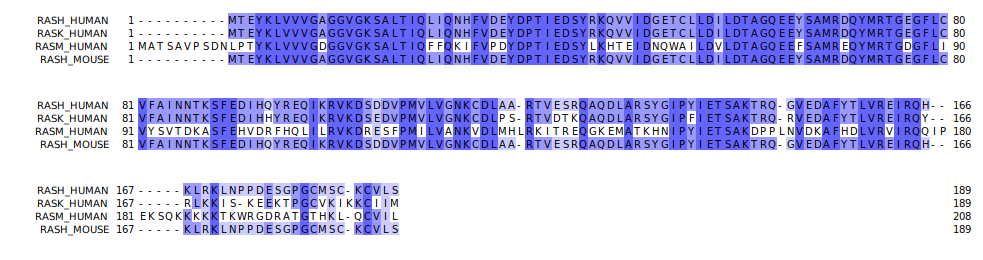
\includegraphics{pic/msa.pdf}
\caption{\label{fig:unnamed-chunk-9}Multiple sequence aligment of RAS
protein family members.}
\end{figure}

Software for MSA:

\begin{itemize}
\tightlist
\item
  MAFFT
\item
  Clustal (Classic)
\item
  MUSCLE
\end{itemize}

\section{Tree methods}\label{tree-methods}

Sequence aligment methods give us information about the similarity
between different sequences. Some sequences are more similar to one
another than to other sequences. Although this information is somwhat
visible in the MSA, it is difficult to visualize complex similarity
relationships when many sequences are considered. To help with this
problem tree visualization methods can be useful. Tree methods use a
distance matrix, e.g.~derived from pairwise sequence aligment of a set
of sequences, and constructs a binary tree in which proteins closer in
the tree are more similar. For example, take a look at the tree shown in
Figure \ref{fig:tree-ras} for the 4 RAS proteins.

\begin{figure}
\centering
\includegraphics{pic/tree_ras.pdf}
\caption{\label{fig:tree-ras}Phylogenetic tree of 4 RAS proteins.}
\end{figure}

\section{Domains and motifs}\label{domains-and-motifs}

Biological sequences contain regions of high similarity to other similar
regions in other proteins. Sometimes this regios are small, accounting
for a few aminoacids, and they are typically named \emph{motifs}. In
other cases the conserved regions are larger, and then are called
\emph{domains}. Domains are sometimes associated with some structurally
motivated definition of domain. Sometimes however, the distinction
between these two types of conserved regions is ambigous.

Motifs and domains can be identified by using the information from a
MSA. This is the approach followed in the Pfam database. Sections of
MSAs containing the domain of interest are manually curated. These are
used to train a Hidden Markov Model (HMM) that learns how to recognize
the same domain in other sequences. With that model, we can identify all
sequences in a database containing that particular domain.

The software HMMER implements HMM for the analysis of biological
sequences. It can learn models representing motifs, domains or entire
sequences. These models are used to search for sequences matching the
models in databases. It can also be used to annotate the domains/motifs
present in a sequence using a database of domains. PFAM uses HMMER and
manually curated MSA of domains to generate a database of protein
families (PFAM). The use of HMM for sequence alignment is described in
detail in the excellent book
\protect\hyperlink{biological-sequence-analysis-probabilistic-models-of-proteins-and-nucleic-acids}{Biological
sequence analysis: Probabilistic models of proteins and nucleic acids}.

\section{Phylogenetics}\label{phylogenetics}

Biological sequences with a commoen evolutionary origin are called
homologs. Homolog sequences found in different species are called
orthologs. Homologs within the same species (i.e.~originated by e.g.~a
gene duplication event) are called paralogs. Because of the shared
ancestry homologs share similarity at the sequence level. The closer
homologs, i.e.~the less time has passed since the two sequences
diverged, the more similar the two sequences will be. Therefore,
sequence similarity is often used as evidence for homology, i.e.~common
ancestry. Here we do not get into the problem of phylogenies but a good
starting point is the classic
\protect\hyperlink{molecular-evolution-and-phylogenetics}{Molecular
evolution and phylogenetics} by M. Nei, creator of the popular
Neighbor-Joining method for tree reconstruction.

\chapter{Omics analysis}\label{omics-analysis-1}

This chapter gives a brief introduction on the most common omics
technologies.

\section{Introduction}\label{introduction}

What is omics? In the last 20 years there has been an explosion of words
ending in \textasciitilde{}ome and \textasciitilde{}omics in the
scientific literature. All these words probably derive from the word
genome and genomics. The definition for genome in a classic textbook in
Biology says: ``Genome is the complete set of genes of an organism''.
Genomics, would be the science that studies the genome.

In a similar way, all the RNA molecules expressed in a cell at a
particular time is called transcriptome. For all the proteins expressed
in a cell we use proteome. For all the metabolites we use metabolome,
and so on. The ome word is also used to describe the complete set of
other ``things'' that are not molecules but some kind of property,
feature or virtually almost anything. For example, interactome may refer
to the complete set of interactions between molecules in the cell.
Extensions of this terminology have resulted in the appearance of terms
like phenome, diseasome, and so on. The technologies used to study
``omes'' are called ``omics''. For example, transcriptomics is the field
that studies the transcriptome. Proteomics is the study of the proteome,
etc. This leads to a whole world of omics technologies.

\begin{figure}
\includegraphics[width=19.78in]{pic/omics_1} \caption{A world of OMICS technologies.}\label{fig:omics-1}
\end{figure}

Let's look into the basic idea behind one of these technologies and what
kind of information they allow us to obtain. For example, here we have
one cell before and after exposure to some stimulus. Transcripts are
represented by these ribbons, each color being a different transcript.
Imagine we are interested on the effect of some chemical on our cells.
We hypothesize that the expression of some genes may be altered by the
effect of the stimulus, but we do not know whether this is true or what
genes may be altered. We decide to do transcriptomics, or gene
expression profiling, to identify which genes are affected. Here we can
see the result from such experiment. In this hypothetical scenario gene
1 has two transcripts, but only the first one is downregulated, i.e.~its
expression is reduced after exposure to the stimulus. Gene 4 has one
transcript that is upregulated, i.e.~its expression is increased by the
stimulus. Other transcripts seem to be unchanged. The expression level
for all transcripts at a given condition is called the expression
profile. By comparing expression profiles we can reveal which genes are
altered between the different conditions. These are called
differentially expressed genes. One of the goals of transcriptomics is
to identify DEGs between different experimental conditions (for example,
between control and treatment, patient and disease, etc.).

\begin{figure}
\includegraphics[width=19.24in]{pic/omics_2} \caption{Rationale behind OMICS technologies.}\label{fig:omics-2}
\end{figure}

Existing omics technologies can be roughly divided into three
categories: microarray based, next generation sequencing approaches (or
NGS) and mass-spectrometry methods (or MS). We will briefly describe
some of these techniques in the following videos.

\begin{figure}
\includegraphics[width=20.82in]{pic/omics_3} \caption{Classification of OMICS technologies.}\label{fig:omics-3}
\end{figure}

\section{Microarrays}\label{microarrays}

\subsection{Expression microarrays}\label{expression-microarrays}

Microarrays were arguably the first of the ``omics'' technologies,
starting a new generation of high-throughput analyses. This type of
exploratory analysis enables the generation of new hypotheses that can
be further tested, becoming one important source of knowledge discovery.
Microarrays were the first technology to allow this and currently there
is a wealth of experimental data available in public databases. There
are over 50,000 samples for expression microarrays deposited in the NCBI
gene expression omnibus (Figure \ref{fig:geo}).

\begin{figure}
\centering
\includegraphics{pic/geo_total.pdf}
\caption{\label{fig:geo}Number of total submissions for the top 4
technologies.}
\end{figure}

Microarrays are basically made of a solid surface with short
oligonucleotides attached to it (see Figure \ref{fig:microarray}). Each
oligonucleotide has a specific sequence, complementary to a particular
gene transcript. This makes the oligonucleotide a probe for the
expression level of the target transcript. The solid surface is divided
into regions forming an array. Each region has attached the same
oligonucleotide and therefore measures the expression of a single
transcript.

\begin{figure}
\includegraphics[width=18.74in]{pic/microarray} \caption{Microarrays are made of oligonucleotide probes attached to a solid surface.}\label{fig:microarray}
\end{figure}

Here we can see a typical microarray experiment protocol in more detail
(Figure \ref{fig:microarray-workflow}). The RNA extracted from the
target cells is converted into cDNA using nucleotides with a
fluorescence molecule attached. A hybridization reaction is performed to
allow the labelled cDNA to bind to its complementary probes. The
location of the hybridized probes is revealed by exciting the array with
a laser. Only those regions with cDNA bound will emit fluorescence upon
stimulation with the laser. Because the location and sequence of the
oligonucleotides are known, the location of the fluorescence will tell
us which transcript has been detected. Image analysis is performed to
quantify the signal associated with each probe, obtaining an estimate of
the transcript's expression level. Analysis of the raw data involves
preprocessing of the intensities (usually background correction and
normalization) and statistical analysis. Variants of this basic protocol
exist that use different labeling approaches, detection methods,
amplification of original RNA, etc.

\begin{figure}
\includegraphics[width=20.07in]{pic/microarray_workflow} \caption{Summary of typical microarray workflow.}\label{fig:microarray-workflow}
\end{figure}

\subsection{Analysis of microarray
data}\label{analysis-of-microarray-data}

Once the hybridization of the samples and microarrays is finished, we
need to measure the signal. This is done by exciting the microarray with
a laser and quantifying the fluerescence light emited. An image of the
microarray is then generated.

In the image only the regions of the microarray where the cDNA has
hybridized will emit light, so we can identify the probes by considering
the position of the emited light. The intensity of the light is
proportional to the amount of cDNA in the original sample complementary
for each probe. So it becomes an estimate of the expression level.

Typically this quantification process is automated and done by the
company or service performing the microarray experiment. So our data
corresponds with a file containing information about each of the probes
in the array and the raw signal (intensity) of the probe, plus some
estimate of the noise associated with each probe. From here, the
following steps are necessary:

\begin{enumerate}
\def\labelenumi{\arabic{enumi}.}
\tightlist
\item
  Load the data into the analysis software (e.g.~into R).
\item
  Preprocess the microarray signal.
\item
  Background correction.
\item
  Normalization.
\item
  Summarization (for Affymetrix microarrays).
\item
  Statistical analysis.
\item
  Writing report sumarizing the results.
\end{enumerate}

For example, here we can se the output of some microarray platform. The
files contain information about each probe position and the intensities.

\begin{verbatim}
[CEL]
Version=3

[HEADER]
Cols=602
Rows=602
TotalX=602
TotalY=602
OffsetX=0
OffsetY=0
GridCornerUL=234 232
GridCornerUR=3844 228
GridCornerLR=3847 3838
GridCornerLL=236 3842
Axis-invertX=0
AxisInvertY=0
swapXY=0
DatHeader=[0..24458]  Madrid pool TX+T3
Algorithm=Percentile
AlgorithmParameters=Percentile:75;CellMargin:2;OutlierHigh:1.500;OutlierLow:1.004

[INTENSITY]
NumberCells=362404
CellHeader=X    Y       MEAN    STDV    NPIXELS
  0       0     114.0   16.4     16
  1       0     8715.8  982.2    16
  2       0     137.3   18.5     16
  3       0     9857.0  1267.9   16
  4       0     65.3    13.3     16
  5       0     121.3   16.6     16
  6       0     8474.8  1411.3   16
  7       0     129.8   27.2     16
  8       0     8462.5  1526.1   16
  9       0     130.8   25.6     16
 10       0     9004.8  1564.8   16
 11       0     120.3   15.3     16
 12       0     9083.0  1590.8   16
 13       0     117.0   21.2     16
 14       0     9177.3  1692.9   16
 15       0     123.0   15.7     16
 16       0     9258.0  1606.6   16
 17       0     116.8   19.3     16
 18       0     9016.0  1662.7   16
 19       0     124.3   22.4     16
\end{verbatim}

\section{Next-generation sequencing}\label{next-generation-sequencing}

An important limitation of microarrays is that they are based on
oligonucleotide probes for detecting expression. This means microarrays
can only detect molecules for which a probe exists in the array. The
probes in a microarray are based on our knowledge of the genome's
sequence at the time of microarray design. Because our knowledge is not
perfect, microarrays often contain probes measuring things different to
what were originally intended. This may lead to incorrect conclusions if
the information about the most likely target sequence is not up to date.
Instead of using a probe to quantify the presence of a DNA or RNA
molecule, why not just sequence the molecule? The problem was that
existing sequencing technology was slow and expensive. This motivated
the development of so called next generation technologies, or NGS.

\subsection{RNA-seq}\label{rna-seq}

Let's look into the fundamental concept behind all NGS technologies from
the perspective of transcriptomics (Figure \ref{fig:ngs}). Imagine this
gene containing one intron and both 5' and 3' UTRs, and is transcribed
into a messenger RNA. The RNA is extracted from the cell and converted
into cDNA. This cDNA is used in microarray technology for the
hybridization reaction. In NGS however, the cDNA is ligated to
sequencing primers, and sequencing produces a set of short reads. Then,
this reads are mapped back using sequence alignment, to some reference
genome. The location and number of reads will reveal, after correcting
from biases like sequencing depth and transcript length, which genes are
being expressed and their abundance levels. There are many applications
of NGS technologies. Next we will review two of the most popular.

\begin{figure}
\includegraphics[width=19.79in]{pic/ngs} \caption{Summary of rationale behind NGS technologies.}\label{fig:ngs}
\end{figure}

The most popular application of NGS technologies is RNA-seq, a
technology to measure the transcriptome (Figure \ref{fig:ngs-rnaseq}).
This slide shows a summary of the typical RNA-seq protocol.

\begin{enumerate}
\def\labelenumi{\arabic{enumi}.}
\item
  Isolate and fragment the RNA.
\item
  A sequencing library is generated by converting the fragmented
  molecules into double stranded cDNA and ligating sequencing primers to
  the ends.
\item
  The cDNA library is sequenced, resulting in a lot of oligonucleotide
  sequences called ``reads''.
\item
  The reads are aligned to a reference genome. The coverage at each
  genome location is defined as the number of overlapping reads. This
  density is proportional to the original molecule's concentration.
  Therefore, molecules found at higher concentrations will show larger
  ``peaks''.
\item
  Computational methods are used to quantify the peaks overlapping gene
  sequences. Statistical methods are used to identify genes with
  differences in expression level.
\end{enumerate}

Because we are not limited to pre-specified sequence probes we can use
the NGS data to detect the expression of alternative splice variants,
non-coding RNAs, genetic variants (or SNPs) and even the expression of
uncharacterized transcripts. Also, if the reference genome information
is updated, the original data can be realigned, never becoming obsolete
and possibly revealing additional information. This versatility
increases dramatically the amount of information that can be obtained
from a single experiment, making RNA-seq one of the most widely used
omics technologies.

\begin{figure}
\includegraphics[width=18.49in]{pic/ngs_rnaseq} \caption{Summary of typical RNA-seq workflow.}\label{fig:ngs-rnaseq}
\end{figure}

\subsection{Example: Stat3 expression in macrophages exposed to
IL10}\label{example-stat3-expression-in-macrophages-exposed-to-il10}

In the following example we will look into an RNA-seq experiment in more
detail. Figure \ref{fig:stat3-rnaseq-1} shows the mouse Stat3 locus
including the exon/intron structure of the different transcripts as
yellow boxes and lines. You can see also other genes nearby, like
Stat5a. The expression level in resting and IL10 stimulated macrophages
is shown as the peaks overlapping with the exons.

\begin{figure}
\includegraphics[width=22.53in]{pic/stat3_rnaseq_1} \caption{Expression of Stat3 in macrophages exposed to IL10.}\label{fig:stat3-rnaseq-1}
\end{figure}

Those peaks represent the density of reads mapping to the genome (Figure
\ref{fig:stat3-rnaseq-2}). The expression level can be computed from the
area of the peaks. Here we see that the expression level of Stat3 is
increased in IL10 treated macrophages. From this picture we can also see
some of the difficulties found when interpreting this type of data. For
example, which of all the Stat3 transcripts are expressed and which are
regulated? Answering this question requires more sophisticated analysis
and possibly additional experiments designed specifically to gather
supporting evidence.

\begin{figure}
\includegraphics[width=20.85in]{pic/stat3_rnaseq_2} \caption{Expression of Stat3 in macrophages exposed to IL10.}\label{fig:stat3-rnaseq-2}
\end{figure}

In Figure \ref{fig:stat3-rnaseq-3} we can see more details for one of
the samples, with the coverage and the aligned reads below. These dense
grey boxes are the actual sequenced reads.

\begin{figure}
\includegraphics[width=20.83in]{pic/stat3_rnaseq_3} \caption{Expression of Stat3 in macrophages exposed to IL10.}\label{fig:stat3-rnaseq-3}
\end{figure}

Let's take a closer look to this region near the first exon (Figure
\ref{fig:stat3-rnaseq-4}). You can see here this boxes indicating the
length of the reads and the arrowed end the strand to which they align.
If we take an even closer look we can see now the reads in more detail.
From this picture you can verify that the coverage is the number of
reads overlapping at each genomic location. Here the grey boxes indicate
that the read sequence matches that of the reference genome to which
they have been aligned. Some of these reads locations, however, show
mismatches. These are probably sequencing errors, but if a location
shows a mismatch consistently found in all reads it will suggest a SNP
in the assayed specimen compared to the reference genome.

\begin{figure}
\includegraphics[width=20.83in]{pic/stat3_rnaseq_4} \caption{Expression of Stat3 in macrophages exposed to IL10.}\label{fig:stat3-rnaseq-4}
\end{figure}

\subsection{ChIP-seq}\label{chip-seq}

Another popular NGS technology is ChIP-seq, which stands for chromatin
immunoprecipitation followed by NGS sequencing. In ChIP-seq we aim to
identify protein-DNA interactions. That is, we want to know the sequence
of the DNA to which a DNA-binding protein binds. This information is
critical to understand gene regulatory programs. For example, gene
transcription is regulated by transcription factors that bind to
specific regions in the genome, including gene promoters and enhancers.
Also, histones represent another type of DNA binding proteins with
important roles in the regulation of gene expression.
Posttranscriptional histone modifications, like acetylation,
methylation, and others, are associated with regulatory outcomes, like
expression activation and repression. ChIP-seq enables to study many of
these patterns at genome wide scale.

The basic ChIP-seq protocol is shown in Figure \ref{fig:ngs-chipseq}.
First, proteins are fixed to the DNA with, e.g.~formaldehyde. Then, the
chromatin is fragmented, leading to many small fragments free of
proteins and some with proteins bound. Among the later ones, some will
be bound to the target protein, that can be a transcription factor or a
histone with some particular modification like H3K9me3 (tri-methylation
of lysine in position 9 of the histone H3). Next, we use an antibody
against the target protein for an immunoprecipitation, which allows us
to obtain the proteins and the DNA sequences they are bound to. Then we
remove the fixation and isolate the DNA. The rest of the protocol, cDNA
library construction and sequencing are performed similarly to RNA-seq.
Sequencing will produce sequence reads that can be aligned to the
reference genome. The read peaks accumulating in DNA loci will reveal
where the target protein was bound. Computational methods are used to
identify and quantify the peaks. Statistical analysis will help us
determine if there is differential binding between experimental
conditions.

\begin{figure}
\includegraphics[width=19.07in]{pic/ngs_chipseq} \caption{ChIP-seq workflow.}\label{fig:ngs-chipseq}
\end{figure}

\subsection{Example: Stat3 binding in macrophages exposed to
IL10}\label{example-stat3-binding-in-macrophages-exposed-to-il10}

In the following example we can see an application of ChIP-seq to
identify the binding locations of the transcription factor Stat3 in
macrophages after exposure to Il10. As before, the Stat3 locus in the
mouse genome is shown, together with the coverage for the Stat3 ChIP-seq
experiment. We can see that Stat3 binds to its own promoter upon Il10
treatment, suggesting that it regulates its own expression.

\begin{figure}
\includegraphics[width=23.21in]{pic/stat3_chipseq} \caption{Stat3 binding profile around the Stat3 locus}\label{fig:stat3-chipseq}
\end{figure}

An important limitation of ChIP-seq is that it can only identify binding
sites for a single TF or histone modification at a time. Another problem
is that in eukaryotes, enhancers can be located far away from the genes
they regulate, hampering the assignment of TF binding to target genes.
Finally, the observation of protein binding to DNA does not demonstrate
its functional relevance, which requires additional functional
experiments.

\subsection{Other NGS technologies}\label{other-ngs-technologies}

Other NGS technologies are becoming popular in recent years. For
example, TSS-seq and CAGE-seq are technologies that identify the 5' cap
structure of the processed mRNA, revealing the location of active
promoters. Other technologies are able to reveal information about the
chromatin. Chromatin accessibility can be assayed by means of either
DNaseI digestion or by transposase reaction. In both cases the enzymes
have a preference to react with open chromatin regions, with regions of
close chromatin or protected by the binding of proteins being more
resilient. This enables to map open chromatin and even the location of
nucleosomes and binding of TFs if enough sequencing depth is performed.
Nucleosome location can be more directly assayed by using the Mnase-seq
protocol. Finally, the methylation of the DNA can be assayed by
bisulfite sequencing.

\section{Mass spectromics methods}\label{mass-spectromics-methods}

Studying transcriptional regulation is one important part for
understanding the cell's phenotype. But some of the transcribed genes
will produce proteins that engage in diverse functions in the cell,
including signaling pathways that regulate the cell's behavior and
enzymes that regulate metabolic pathways. Therefore, the other important
part to understand the cell's phenotype are the proteome and metabolome.
For studying the proteome mass-spectrometry (or MS) approaches have been
fundamental. Here we will focus on the use of MS approaches for
proteomics.

MS uses the mass-to-charge ratio to identify and quantify chemical
molecules. MS is used not only to quantify protein expression, but also
post-translational modifications like phosphorylation or ubiquitination,
and protein-protein interactions.

\subsection{MS}\label{ms}

The general proteomics protocol requires digesting the proteins into
fragments (peptides). These will be initially separated by liquid
chromatography (LC) coupled to MS. This will lead to peptide separation
but identification requires another round of fragmentation followed by
MS. Each peptide produces a distinct spectrum, which is compared against
a database linking spectra to peptide sequences. The identified peptides
are then mapped to a protein database to identify the proteins they came
from. The number of mapping peptides will be proportional to the
original abundance of the proteins, enabling their quantification.

\begin{figure}
\includegraphics[width=16.28in]{pic/ms} \caption{Workflow for MS proteomics.}\label{fig:ms}
\end{figure}

\subsection{AP-MS}\label{ap-ms}

Protein interactions are fundamental in regulating cellular pathways,
and they play as well important roles in immunology. To obtain
protein-protein interaction information we can use a modified MS
protocol called AP-MS (affinity purification followed by MS). Similar to
ChIP-seq, the first step is to crosslink interacting proteins together
with formaldehyde. Next, we isolate the complexes with an antibody
against the target protein, also call the bait. Then, crosslinking is
reversed, the proteins are digested and LC-MS/MS performed in the usual
way. Mapping the peptides to the proteome will identify which other
proteins where interacting with our target protein. AP-MS can only assay
the interactome around the target protein. Also, it does not identify
direct interactions, but proteins that are part of the same protein
complex.

\begin{figure}
\includegraphics[width=22.72in]{pic/ap-ms} \caption{Workflow for AP-MS proteomics for identifying protein-protein interactions.}\label{fig:ap-ms}
\end{figure}

\section{Single cell omics}\label{single-cell-omics}

So far we have assumed that in each omic experiment we obtain a tissue
sample, or perhaps isolate the cell type of interest with FACS and then
perform the analysis on the bulk of cells. An experiment performed in
this way reveals information about (in the case of transcriptomics) the
average expression level of all cells in the bulk. In general, this
approach is valid if we believe that most of the cells in the population
are similarly and that they behavior is homogeneous. However, recent
evidence shows that even in seemingly homogenous populations, there is
substantial heterogeneity in the expression levels of genes and
proteins. This is even more dramatic in populations where a few cells
are regulated distinctly and initiate changes that will drive future
responses. For example, in the lymph node there are many naive T cells
but only the ones in contact with their specific antigen will be
activated and mature into effector cells. Because the associated changes
occur in a very limited number of cells, that information may be lost in
the averaging resulting from analyzing bulks of cells. This is the
motivation behind the field of single cells omics. The foundation of
single cell omics is almost identical to what we have seen so far. The
main difference is that these omics technologies are applied to each
cell individually, requiring of methods to manipulate and extract the
target material from single cells in parallel and efficiently. Another
challenge is the analysis of this type of data. The data resulting from
single cell omics is multivariate in nature and specialized methods are
required for their interpretation.

\begin{figure}
\includegraphics[width=15.22in]{pic/ngs_sc} \caption{Single cell omics captures the stochastic nature of biological processes}\label{fig:sc}
\end{figure}

The field of single cell omics is in constant development and new or
improved methodologies appear increasingly. For transcriptomics the use
of microfluidic reaction chambers enables single cells to be subjected
to RNA-seq protocols. Another methodology is Fluorescence based flow
cytometry (FBFC), which enables to quantify the amount of proteins using
fluorophores attached to antibodies. However, because spectral overlap,
the maximum number of proteins that can be measured simultaneously is
limited. A modification of this technology known as mass cytometry tags
antibodies with rare isotopes and uses mass spectrometry to identify
proteins. This technique highly improves the dimensionality by
increasing the number of proteins and conditions that can be analyzed
simultaneously.

\section{Batch effects}\label{batch-effects}

An important topic related to omics analyses is batch effects. The issue
is very eloquently presented in a 2010 Nature paper by Rafael Irizarry
\emph{Tackling the widespread and critical impact of batch effects in
high-throughput data}. Batch effects are variation in our data due to
e.g.~laboratory conditions, reagent lots and personal differences.
Importantly, when these effects are correlated with the variables under
study (e.g.~treatment in a study that aims to assess the effect of the
treatment) batch effects can put into question the conclusions from our
studies. The best way to prevent batch effects is by designing
experiments in a way that avoids correlation between potential sources
of batch effect and the main variables under study. This may be
challenging to do in very complicated studies or when using human
samples, when the collection and time of experiment often cannot be
controlled. Although batch effects are also found in low throughtput
technologies, high-throughput technologies contain information that can
help researchers remove their contribution. For this, the use of
appriate statistical techniques is necessary.

\chapter{Bioinformatics resources}\label{bioinformatics-resources}

In this chapter some of the most important Bioinformatics resources are
described. An attempt to organized them by topic is made, but most of
these resources are highly integrated. So, for example, you would thing
that to do a Blast search you need to go to the Blast web page. But you
can also perform Blast searches from the Uniprot and EnsEMBL web pages,
to mention just two. Similarly, most if not all sequence databases link
the associated Gene Ontology information to their sequence entries. This
high degree of integration might make difficult at first to value the
existence of different resources.

\section{Gene Ontology}\label{gene-ontology}

One important difficulty when dealing with Biological structures
(molecules, organelles, etc.) is the vocabulary we use to described
them. As this type of information accumulated different researches would
tend to use slighly different ways to describe the same thing. In other
cases they can use similar words to describe different things. These
nuances make the descriptions often found in publications ambiguous
making it difficult to determine the exact meaning of some assertion.
This difficulty became more prominent once the amount of information
increased dramatically with the advent of omics technologies, and the
information about the biological stuff was the subject of computational
analyses. There was a need for an standardized nomenclature, and that
was the origin of the \href{http://www.geneontology.org}{Gene Ontology}
project. The purpose of the Gene Ontology project is stated in it web
page:

\begin{quote}
The Gene Ontology (GO) project is a major bioinformatics initiative to
develop a computational representation of our evolving knowledge of how
genes encode biological functions at the molecular, cellular and tissue
system levels. Biological systems are so complex that we need to rely on
computers to represent this knowledge. The project has developed formal
ontologies that represent over 40,000 biological concepts, and are
constantly being revised to reflect new discoveries. To date, these
concepts have been used to ``annotate'' gene functions based on
experiments reported in over 100,000 peer-reviewed scientific papers.
\end{quote}

In particular:

\begin{quote}
The Gene Ontology project provides a controlled vocabulary of terms for
describing gene product characteristics and gene product annotation data
from GO Consortium members, as well as tools to access and process these
data.
\end{quote}

\begin{figure}
\includegraphics[width=16.21in]{pic/go_web} \caption{Screenshot of the Gene Ontology home page at http://www.geneontology.org.}\label{fig:go-web}
\end{figure}

\section{Sequence databases}\label{sequence-databases}

\subsection{NCBI}\label{ncbi}

\subsection{EnsEMBL}\label{ensembl}

\href{https://www.ensembl.org}{EnsEMBL} is a database where the genome
information about many species is collected with a focus con comparative
genomics research.

\begin{figure}
\includegraphics[width=17.04in]{pic/ensembl_web} \caption{Screenshot of the EnsEMBL home page at https://www.ensembl.org.}\label{fig:ensembl-web}
\end{figure}

\subsection{Uniprot}\label{uniprot}

The \href{http://www.uniprot.org}{Uniprot} website focuses on
information about protein sequences, including splice forms.

\begin{figure}
\includegraphics[width=16.94in]{pic/uniprot_web} \caption{Screenshot of the Uniprot home page at http://www.uniprot.org.}\label{fig:uniprot-web}
\end{figure}

\section{Gene expression databases}\label{gene-expression-databases}

\subsection{GEO: Gene Expression
Omnibus}\label{geo-gene-expression-omnibus}

The \href{https://www.ncbi.nlm.nih.gov/geo/}{Gene Expression Omnibus
(GEO)} database collects data from high-throughtput experiments
including microarrays and NGS datasets.

\begin{figure}
\includegraphics[width=16.38in]{pic/geo_web} \caption{Screenshot of the GEO home page at https://www.ncbi.nlm.nih.gov/geo/.}\label{fig:geo-web}
\end{figure}

The number of submissions per year for microarrays and RNA-seq continues
to increase.

\begin{figure}
\centering
\includegraphics{pic/geo_year.pdf}
\caption{\label{fig:geo-year}Number of GEO submissions per year for the top
4 technologies.}
\end{figure}

\subsection{ArrayExpress}\label{arrayexpress}

\href{https://www.ebi.ac.uk/arrayexpress/}{ArrayExpress} is the
alternative at the European Bioinformatics Institute.

\begin{figure}
\includegraphics[width=16.51in]{pic/ae_web} \caption{Screenshot of the ArrayExpress home page at https://www.ebi.ac.uk/arrayexpress/}\label{fig:ae-web}
\end{figure}

\section{Pathway databases}\label{pathway-databases}

As information about genes, proteins and metabolites accumulates, it
becomes more and more important to organize this knowledge in a
comprehensive way. We have mentioned how genes and their products
participate in the networks of cellular processes, the cell's pathway.
This network includes metabolic, signaling and gene regulatory networks.
This information is critical to understand the cell's phenotype, but the
accumulated knowledge is daunting. It would benefit to have some central
repository with easily accessible tools that enables to visualize
existing knowledge in an easy way. It would be also very useful if it
was possible to use that information in computer analysis. This is the
motivation behind some of the web resources described below.

\subsection{KEGG}\label{kegg}

KEGG stands for \href{http://www.kegg.jp}{Kyoto Encyclopedia for Genes
and Genomes} (Figure \ref{fig:kegg-web}). Is an integrative resource
with information about matabolic and signaling pathways in different
species, from bacteria and archaea to mammals.

\begin{figure}
\includegraphics[width=10.4in]{pic/kegg_web} \caption{Screenshot of the KEGG home page at http://www.kegg.jp.}\label{fig:kegg-web}
\end{figure}

\subsection{Reactome}\label{reactome}

\section{Domain databases}\label{domain-databases}

\subsection{Pfam}\label{pfam}

\href{http://pfam.xfam.org}{Pfam} is a database of protein domain
families.

\begin{quote}
Proteins are generally comprised of one or more functional regions,
commonly termed domains. The presence of different domains in varying
combinations in different proteins gives rise to the diverse repertoire
of proteins found in nature. Identifying the domains present in a
protein can provide insights into the function of that protein.

The Pfam database is a large collection of protein domain families. Each
family is represented by multiple sequence alignments and a hidden
Markov model (HMMs).
\end{quote}

\begin{figure}
\includegraphics[width=16.97in]{pic/pfam_web} \caption{Screenshot of the Pfam home page at http://pfam.xfam.org.}\label{fig:pfam-web}
\end{figure}

\section{Motif databases}\label{motif-databases}

\subsection{Jaspar}\label{jaspar}

\href{http://jaspar.genereg.net}{Jaspar} is a database for transcription
factor DNA binding motifs.

\begin{figure}
\includegraphics[width=17.03in]{pic/jaspar_web} \caption{Screenshot of the Jaspar home page at http://jaspar.genereg.net.}\label{fig:jaspar-web}
\end{figure}

\section{Interaction networks}\label{interaction-networks}

Information about protein-protein interactions has grown incredibly due
to advances in MS in combination with affinity purification methods.
There are several databases integrating existing information. Two
resources will be highlighted here: BioGRID and STRING.

\subsection{BioGRID}\label{biogrid}

\href{https://thebiogrid.org}{BioGRID} focuses on storing information
about PPIs for which experimental evidence exists.

\begin{figure}
\includegraphics[width=14.17in]{pic/biogrid_web} \caption{Screenshot of the BioGRID home page at https://thebiogrid.org.}\label{fig:biogrid-web}
\end{figure}

\subsection{STRING}\label{string}

STRING combines experimental and computational evidence to infer PPIs.

\begin{figure}
\includegraphics[width=14.21in]{pic/string_web} \caption{Screenshot of the STRING home page at https://string-db.org.}\label{fig:string-web}
\end{figure}

\section{Bioformatics software}\label{bioformatics-software}

\subsection{Blast}\label{blast-1}

The \href{https://blast.ncbi.nlm.nih.gov}{Blast} web page at NCBI is the
main point of access to this versitile tool. It can be used to search
for sequence similarity against any of the sequence databases at the
NCBI.

\begin{figure}
\includegraphics[width=16.83in]{pic/blast_web} \caption{Screenshot of the Blast home page at https://blast.ncbi.nlm.nih.gov.}\label{fig:blast-web}
\end{figure}

\subsection{Jalview}\label{jalview}

\href{http://www.jalview.org}{Jalview} is a software for sequence
analysis. It can visualize sequences, submit them to multiple sequence
aligment servers, visualize the resulting MSA, create basic phylogenetic
trees and visualize associated structures.

\begin{figure}
\includegraphics[width=16.9in]{pic/jalview_web} \caption{Screenshot of the Jalview home page at http://www.jalview.org.}\label{fig:jalview-web}
\end{figure}

\subsection{MEME}\label{meme}

The \href{http://meme-suite.org}{MEME-suite} is a collection of tools
for the discovery of motifs in proteins, DNA and RNA sequences. If can
find de-novo motifs (e.g.~MEME) or search for known motifs from a motif
database (e.g.~MAST, FIMO, etc.)

\begin{figure}
\includegraphics[width=11.78in]{pic/meme_web} \caption{Screenshot of the MEME-suite home page at http://meme-suite.org.}\label{fig:meme-web}
\end{figure}

\subsection{Bioconductor}\label{bioconductor}

\subsection{Cytoscape}\label{cytoscape}

\section{File formats}\label{file-formats}

\subsection{FASTA}\label{fasta}

FASTA is a very simple file format used to store information about
biological sequences, including protein, DNA and RNA. Each entry
consists of the \texttt{\textgreater{}} character followed by a sequence
\emph{Id} and a description, separated from the \emph{Id} by a space
character. The sequence itself goes in the next lines. Often FASTA files
are formatted with a maximum number of residues per line (e.g.~60),
which helps when visualizing the information in a regular text editor.

\begin{verbatim}
>seq1 This is seq1
AGTTAGGATTTGCGCCATT
\end{verbatim}

\chapter{Reproducible research}\label{reproducible-research}

An important topic in Bioinformatics as a research tools is
reproducibility. Bioinformatics pipelines typically require numerous
steps in which different parameters can change and affect the results.
Also, software sometimes gets updated and not always updates are
backbard compatible in the sense that changes in the underlying
algorithms results in changes in the results. It is desirable to use a
system that encourages transparent reports that enable to repeat the
steps used during a particular analysis in order to reproduce the
reported results. In this chapter we briefly describe some of the tools
used by the modern Bioinformatician to accomplish this.

\section{Git}\label{git}

\subsection{Github}\label{github}

\section{Literate programming}\label{literate-programming}

\subsection{RMarkdown notebooks}\label{rmarkdown-notebooks}

\subsection{Jupyter notebooks}\label{jupyter-notebooks}

\chapter{Learning Bioinformatics}\label{learning-bioinformatics}

\section{Books}\label{books}

\subsection{Sequence analysis}\label{sequence-analysis-1}

\hypertarget{blast-an-essential-guide-to-the-basic-local-alignment-search-tool}{\subsubsection*{BLAST:
An essential guide to the Basic Local Alignment Search
Tool}\label{blast-an-essential-guide-to-the-basic-local-alignment-search-tool}}
\addcontentsline{toc}{subsubsection}{BLAST: An essential guide to the
Basic Local Alignment Search Tool}

Introductory book to the topic of sequence aligments in general and
Blast in particular. Includes Perl code.

\begin{figure}
\includegraphics[width=6.94in]{pic/blast_book} \caption{Blast. Ian Korf, ... O'Reilly, 2003}\label{fig:unnamed-chunk-10}
\end{figure}

\hypertarget{biological-sequence-analysis-probabilistic-models-of-proteins-and-nucleic-acids}{\subsubsection*{Biological
sequence analysis: Probabilistic models of proteins and nucleic
acids}\label{biological-sequence-analysis-probabilistic-models-of-proteins-and-nucleic-acids}}
\addcontentsline{toc}{subsubsection}{Biological sequence analysis:
Probabilistic models of proteins and nucleic acids}

Advance level understanding of the theory of sequence aligment and
Hidden Markov Models (HMM).

\begin{figure}
\includegraphics[width=4.83in]{pic/hmm_book} \caption{Biological sequence analysis: Probabilistic models of proteins and nucleic acids. R. Durbin, S. Eddy, ... Cambridge, 1998}\label{fig:unnamed-chunk-11}
\end{figure}

\hypertarget{molecular-evolution-and-phylogenetics}{\subsubsection*{Molecular
evolution and
phylogenetics}\label{molecular-evolution-and-phylogenetics}}
\addcontentsline{toc}{subsubsection}{Molecular evolution and
phylogenetics}

Introductory level book on the topic of inferring phylogenies from
sequence information.

\begin{figure}
\includegraphics[width=4.75in]{pic/phylogenetics_book} \caption{Molecular evolution and phylogenetics. M. Nei, S. Kumar. Oxford University Press, 2000.}\label{fig:unnamed-chunk-12}
\end{figure}

\subsection{Omics technologies}\label{omics-technologies}

\section{Online resources}\label{online-resources}

\subsection{Learning how to use the command
line}\label{learning-how-to-use-the-command-line}

Sometimes using Bioinformatics tools requires to have some knowledge of
how to use the command line, specially in Linux/Unix environments.
\href{http://linuxcommand.org/index.php}{http://linuxcommand.org} has a
nice introduction to the Linux command line.

Another interesting resource is \url{https://www.codecademy.com},
providing an interactive learning experience. It offers also paid
courses.

\subsection{Support Communities}\label{support-communities}

Learning Bioinformatics, as with any other complex topic, can be
daunting. Often Bioinformatics software come with good and detailed
documentation and. It is also possible to frequently find short
tutorials that can help newcomers get started. It is important to get a
\emph{good} understanding of the methods being used when the goal is to
publish your results. The Bioinformatics community can sometimes help in
the learning process by providing solutions to the most frequently
encountered problems. Here I will highlight some of the most relevant
online communities for the Bioinformatician.

\subsubsection*{Biostars}\label{biostars}
\addcontentsline{toc}{subsubsection}{Biostars}

\href{http://biostars.org}{Biostars} is an online community deboted to
answering questions about \emph{``bioinformatics, computational genomics
and biological data analysis''}. Users can post questions, get answers
in the same post. There is a rating system that enables to give credit
to good questions and answers. It is possible to include comments for
further clarification and discussion.

\subsubsection*{Bioinformatics Stack
Exchange}\label{bioinformatics-stack-exchange}
\addcontentsline{toc}{subsubsection}{Bioinformatics Stack Exchange}

Another useful resource for solving general questions related to
Bioinformatics can be the
\href{https://bioinformatics.stackexchange.com}{Bioinformatics Stack
Exchange} network. These site follows the same phylosohpy of Biostars
(indeed, Biostars originated in the old version of Stack Exchange) but
offers, in my opinion, a better user inteface. The site is still in beta
but most of the Biostars community can be found also in this new site.

\subsubsection*{Bioconductor support
site}\label{bioconductor-support-site}
\addcontentsline{toc}{subsubsection}{Bioconductor support site}

The \href{https://support.bioconductor.org}{Bioconductor support site}
provides support for questions related to the use of Bioconductor, using
a similar interface to Biostars.

\subsubsection*{How to use the support
sites}\label{how-to-use-the-support-sites}
\addcontentsline{toc}{subsubsection}{How to use the support sites}

It is important to remember that online support sites are usually driven
by voluntarees that lend their time and expertise to help others.
Because the number of questions put in one of these support sites can be
very large, it is very helpful if the questions themeselves are written
in a way that simplify the work of those willing to help us with our
doubts. For example, it is important to write simple yet meaningful
titles that summarize what our problem is. This way the community can
easily know if the question is related to a topic about which they have
expertise. When describing your issues, be as explicit as possible. And
whenever possible, include a
\href{https://en.wikipedia.org/wiki/Minimal_Working_Example}{minimal
reproducible example}. This is particularly important if you have
problems with programming code but it can also apply to using a web
server. For example, if you had some problem using a web server to
generate a sequence aligment, include all the steps you performed to
obtain the error (if any) you obtained. If possible, when needed,
include a minimal example dataset to reproduce the error. In this
example, it could be a small file with a few sequences that trigger the
error.

The particulars will depend of the software and problem you are having.
But as a rule of thumb it is always helpful to put yourself in the place
of those reading your question, and imagining whether that is enough for
them to understand your problem.

\bibliography{book.bib,packages.bib}


\end{document}
